\documentclass[12pt]{article}
\usepackage[utf8]{inputenc}
\usepackage{mathrsfs}
\usepackage[margin=3.0cm]{geometry}
\usepackage[version=4]{mhchem}
\usepackage{booktabs}
\usepackage{indentfirst}
\usepackage{smartdiagram}
\usesmartdiagramlibrary{additions}
\usepackage{verbatim}
\usepackage[dvipsnames]{xcolor}
\def\checkmark{\tikz\fill[scale=0.4](0,.35) -- (.25,0) -- (1,.7) -- (.25,.15) -- cycle;} 
\newcommand{\xdownarrow}[1]{%
  {\left\downarrow\vbox to #1{}\right.\kern-\nulldelimiterspace}}
\newcommand{\xDownarrow}[1]{%
  {\left\Downarrow\vbox to #1{}\right.\kern-\nulldelimiterspace}}
\usepackage{cmap}
\usepackage{lmodern}
\usepackage[T1]{fontenc}
\usepackage{indentfirst}
\usepackage{float}
\usepackage{nomencl}
\usepackage{graphicx}
\usepackage{textcomp}
\usepackage{comment}
\usepackage{setspace}
\usepackage[usenames,dvipsnames,svgnames,table]{xcolor}
%\usepackage[brazil]{babel}
%\usepackage{fullpage}
%\usepackage[margin=4cm]{geometry}
\usepackage{amsmath,amsthm,amsfonts,amssymb,amscd}
\usepackage{lastpage}
\usepackage{enumerate}
\usepackage{fancyhdr}
\usepackage{mathrsfs}
\usepackage{graphicx}
\usepackage{listings}
\usepackage{hyperref}
\usepackage{multicol}
\usepackage{adjustbox}
\usepackage{array}
\usepackage{ragged2e}
\usepackage{arydshln}
\usepackage{multirow}
\usepackage{adjustbox}
%\usepackage{biblatex}
\usepackage{wrapfig}
\usepackage{smartdiagram}
\usepackage{gensymb}
\usepackage{wrapfig,lipsum,booktabs}
%\addbibresource{ref.bib}
\usepackage{dirtytalk}

%\usepackage{natbib}
\usepackage{graphicx}
\newcommand{\blank}[1]{\hspace*{#1}}
\usepackage{caption}

\begin{document}

\begin{center}
    \LARGE{\textbf{FINAL PROJECT}\\
    \textbf{The Moran Model - Neutral Evolution}}\\
    \vspace{2mm}
    \Large{\textit{Computational Methods}}\\
    \large{Prof. Andrea Sánchez-Tapia}\\
    \large{Prof. Sara Mortara}\\
    \vspace{3mm}
    \large{Amanda Araujo Silva\\
    \textsc{2022}}
\end{center}
%\vspace{3mm}

\section{Introduction}
This project aims to investigate concepts in evolutionary dynamics, especially biological effects that arise from stochasticity, such as neutral drift. The goal is to study the Moran model and get an intuition of its behavior and biological implications.

\subsection{Theorical basis}
\indent Evolution dynamics depend on two processes: genetic variability by mutations and changes in the frequency of alleles within the population over time. In a simplistic way, a mutation can be advantageous, disadvantageous, or neutral, in terms of altering the fitness of the individual. The first two's fate is subjected to natural selection, while in the last one alterations in allele frequencies are just due to random processes, called genetic drift. Both cause changes in the frequency of alleles, but while natural selection is directional, genetic drift is driven by stochasticity \cite{duret2008neutral}.\\
\indent The Moran model was proposed in 1958, by the Australian statistician Patrick Moran, and it is the simplest stochastic formulation of finite population evolution. It can describe the probabilistic dynamics of two alleles A and B competing for dominance. The model allows us to ask questions such as how/whether/when a gene is lost in a population. \cite{moran1958random}\cite{nowak2006evolutionary}. 

\subsection{The model}
\indent Assumptions of the Moran model:\\
\indent\indent \checkmark Total size of the population is constant, $N$;\\
\indent\indent \checkmark Composition is fixed in terms of allele variants A and B, no mutations;\\
\indent\indent \checkmark Asexual reproduction;\\
\indent\indent \checkmark Generations overlap.\\

\begin{minipage}{.5\textwidth}
    \indent Frequencies:\\
    \blank{0.5cm} $i \equiv$ absolute frequency of A\\
    \blank{0.5cm} $N - i \equiv$ absolute frequency of B
\end{minipage}
\begin{minipage}{.5\textwidth}
    At each iteration randomly:\\
    \blank{0.5cm} $\bullet$ Choose 1 individual to reproduce\\
    \blank{0.5cm} $\bullet$ Choose 1 individual to replace
\end{minipage}


\subsection{Implementation}

\indent In order to implement the model, the state of the population is tracked by the frequency of allele A, given by $i$, the only stochastic variable of the system. 

\begin{center}
    \begin{minipage}{.5\textwidth}
    \blank{0.5cm} At each iteration, the allele A can gain or lose one unit or stay the same, with the probabilities of changing state given by:
    \begin{center}
        \indent\indent $P_{i, i + 1} = \frac{i}{N}\frac{(N - i)}{N}$\\
        \vspace{2mm}
        \indent\indent $P_{i, i - 1} = \frac{(N - i)}{N}\frac{i}{N}$\\
        \vspace{2mm}
        \indent\indent $P_{i, i} = 1 - P_{i, i + 1} - P_{i, i - 1}$
    \end{center}
    \end{minipage}% This must go next to `\end{minipage}`
    \begin{minipage}{.5\textwidth}
        \centering
        \includegraphics[scale = 0.8]{moran-states.png}
        %\caption{Caption}
        \label{fig:my_label}
    \end{minipage}
\end{center}

\indent In the neutral evolution case, it is assumed that alleles A and B present the same fitness, \textit{i.e.} $P_{i, i + 1} = P_{i, i - 1}$. The decision of which event will take place is made computationally through the use of a uniform number generator.


\section{Results and discussion}

\subsection{Moran model neutral evolution}
\indent The Moran model was implementated in two programming languages, \textit{R} and \textit{Python}. 

\begin{figure}[H]
    \centering
    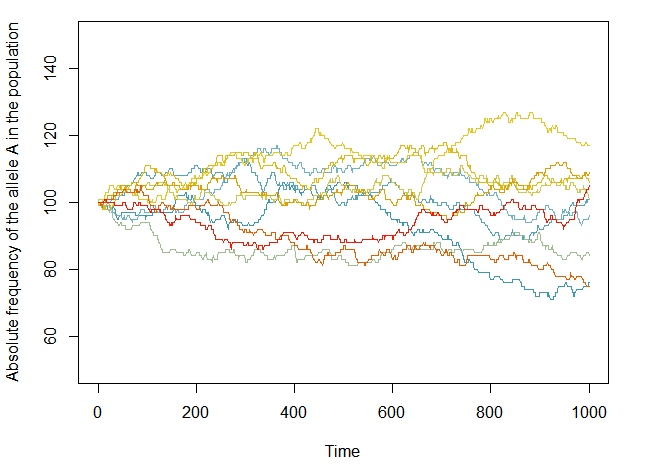
\includegraphics[scale=0.7]{moran-neutral-N1000-i100-t1000-notitle-R.png}
    \caption{Moran process of neutral evolution for a population size $N = 1000$. Initial value of the number of allele A in the polutation $i = 100$. 1000 iterations. 10 independent \textit{R} simulations, each one represent by a different line color.}
    \label{fig:moran-neutral}
\end{figure}

\indent In Fig. (\ref{fig:moran-neutral}) we can see the dynamics of the alleles' proportion within a fixed population size. The system behaves as a \say{random walk}: starting with the same $i$ value leads to different dynamics of allele frequencies within the population. Due to neutral evolution, the chance of allele A or B being chosen at each iteration is the same, reflected in no observation of a preferential direction in the 10 independent runs.


\subsection{Size matters: exploring different population sizes $N$'s}
\begin{figure}[H]
    \centering
    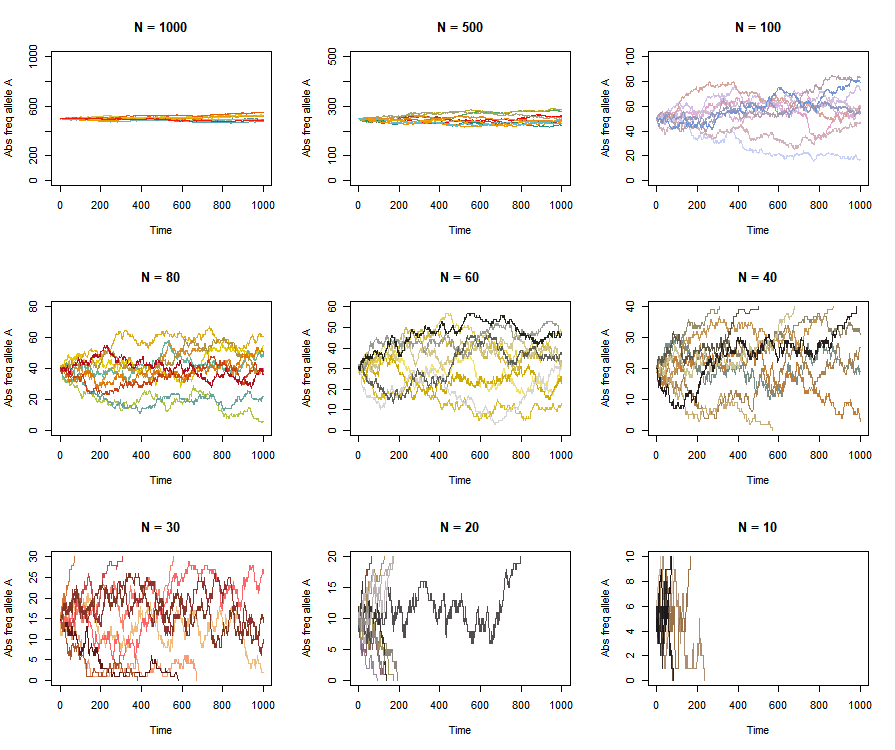
\includegraphics[width = \textwidth]{moran-neutral-N10_1000-i(50)-t1000-3x3-R.png}
    %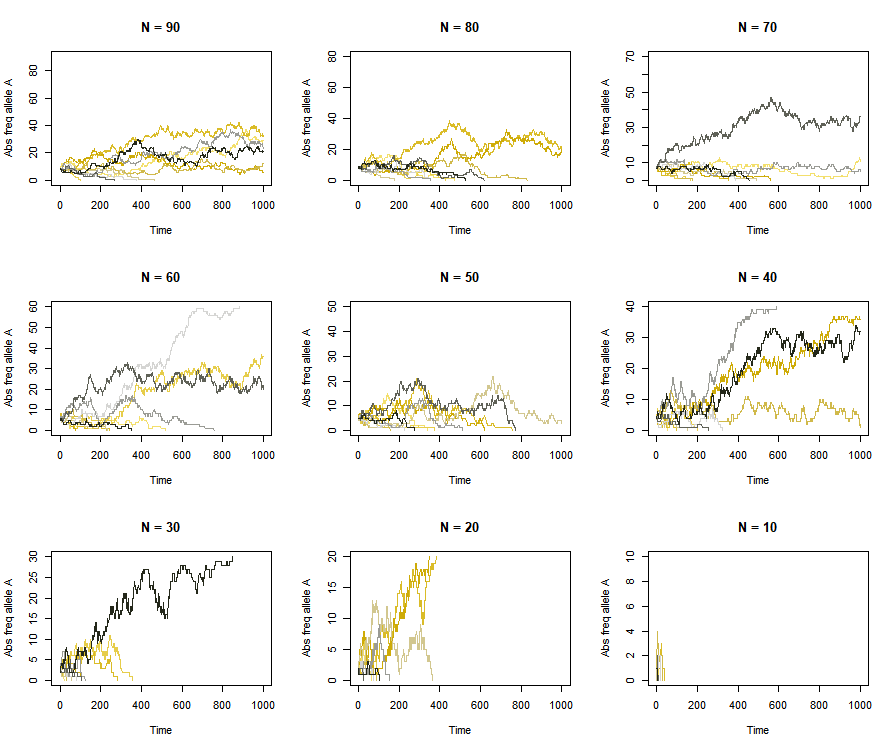
\includegraphics[width = \textwidth]{moran-neutral-N10_90-i(10)-t1000-R.png}
    \caption{Moran process neutral evolution simulated in \textit{R} for different population sizes $N = 1000, 500, 100, 80, 60, 40, 30, 20, 10$. Initial value of the number of allele A in the polutation $i$ corresponding to the proportion of 50\% for all $N$'s. 1000 iterations.}
    \label{fig:diff_sizesN}
\end{figure}
\indent Simulating the model for different population sizes Fig. (\ref{fig:diff_sizesN}), when we can see that the fluctuations affect the systems at different levels. The system presents two absorbing states, 0 and 1, \textit{i.e.} states from which the system cannot leave after reaching it. Biologically, it means the elimination or fixation of the allele, respectively, and that there's no coexistence of alleles. All other states are transient. \\
\indent For larger populations, the transient time is longer; we can see that even after 1000 iterations, in populations with sizes such as $N = 1000, 500, 100$, none of the runs reached the final stage, the effect of $\pm 1$ is less felt by the system. On the other hand, we observe that the smaller the population size, the more notable the effect of stochasticity. For $N \leq 40$ we observe most of the simulations reaching one of the absorbing states, with $\downarrow N$ resulting in shorter mean times to reach the culmination of the evolutionary process.

%\subsection{Exploring different initial values $i$'s}
\subsection{Probability of fixation}

\indent Knowing that the genetic drift leads to one allele dominating over the other, it is worth questioning what would it be the allele's A fixation probability given its initial frequency in the population $i$. 
\begin{figure}[H]
\minipage{0.32\textwidth}
  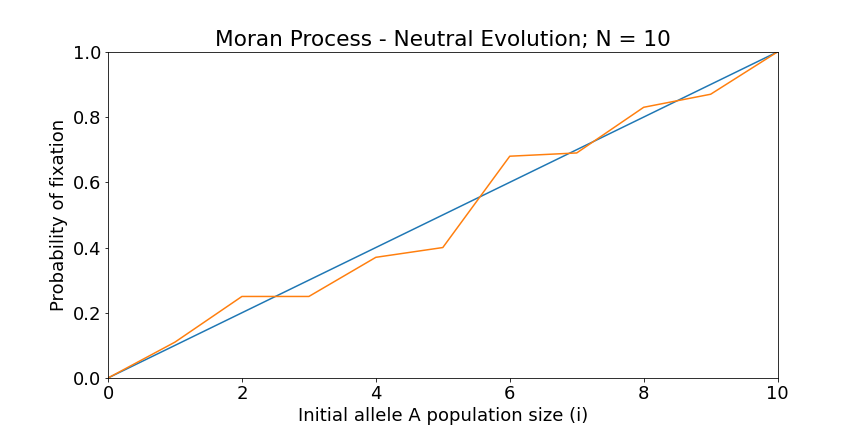
\includegraphics[width=\linewidth]{moran-neutral-N10-Pfixation-Py.png}
\endminipage\hfill
\minipage{0.32\textwidth}
  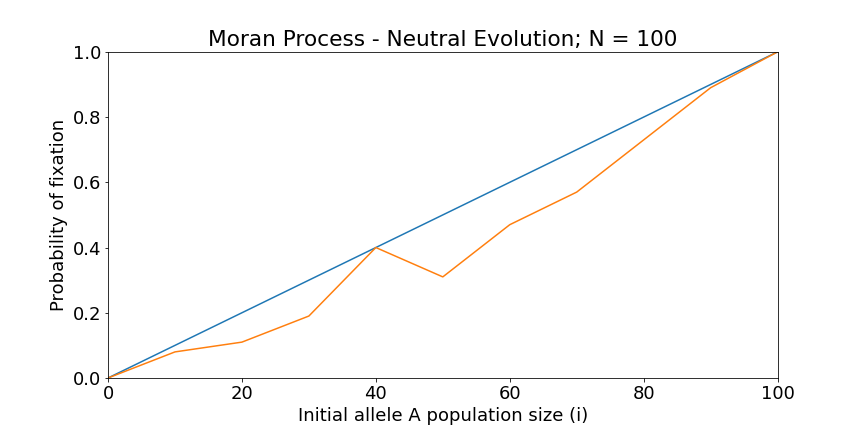
\includegraphics[width=\linewidth]{moran-neutral-N100-Pfixation-Py.png}
\endminipage\hfill
\minipage{0.32\textwidth}%
  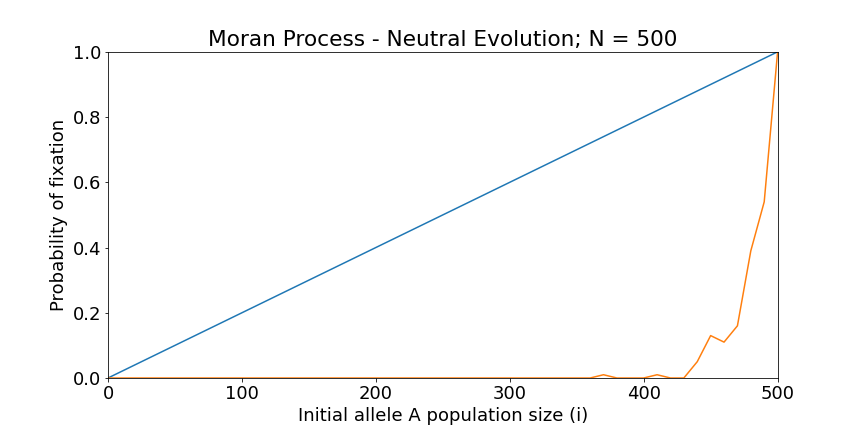
\includegraphics[width=\linewidth]{moran-neutral-N500-Pfixation-Py.png}
  %\caption{A really Awesome Image}\label{fig:awesome_image3}
\endminipage
\caption{Probability of fixation for different population sizes $N = 10, 100, 500$ given the initial frequency of allele $i$. Blue line indicates theoretical probability, orange line the probability obtained after  
simulating the model in \textit{Python} with 10000 iterations, 100 runs for each $i$.}
\label{fig:oi}
\end{figure}
\indent It is deeply related to the initial proximity to the absorbing states, with a fixation probability of $i/N$ (theoretical), but simulating it Fig. (\ref{fig:oi}) we can observe that the result depends on the size of the population, with fluctuations for more or less the theoretical value for small $N$, and the number of iterations: for large $N$ if we don't give it enough time we won't see allele A fixating unless for values of $i$ starting close to 100\% of total population size.

\section{Conclusion}
\indent After all the simulations, we can have as a take-home message that stochastic processes appear in multi aspects of biology, but in evolution, stochasticity is particularly important, yielding to unique mechanisms that can shape evolutionary dynamics.\\
\indent This short project was a way of exercizing the tools and knowledges seen in the Computational Methods course, in the Serrapilhiera/ICTP-SAIFR Quantitative Biology and Ecology Program. It is an Open Science initiative, all the project's codes can be found in: \url{https://github.com/amanda-araujo/stochastic-mathematical-modeling}.


%References
\bibliographystyle{plain}
\bibliography{ref.bib}

\end{document}